\section{Microcontroller}

\subsection{OS}
\subsection{Scheduling}
Det er vigtigt i enhver kode situation, der inkluderer flere tasks, at kunne skifte mellem dem på en fornuftig måde; Dette gøres med en scheduler. Når der skal implementeres en scheduler skal det overvejes hvorvidt det er nødvendigt at lave en designed specielt til projectet, eller om der en en eksisterende der er i stand til at udfører opgaven tilstrækkeligt. I dette project havde vi tre muligheder til rådighed: RTCS, FreeRTOS, og at lave vores egen.
\\
Den simple løsning er at bruge RTCS. Denne er simpel at benytte, og kan godt opfylde de grundlæggende krav vi har til systemet. Dog har denne ikke prioritering, preemption, eller mutex.
\\
Den mere tidskrævende løsning ville være at lave en selv. Dette ville kræve en del tid og mange flerer overvejelser omkring hvilke funktionaliteter der kræves, uden at det ville give den store fordel set i forhold til RTCS.
\\
Den sidste løsning er at benytte FreeRTOS. Denne har meget mere funktionalitet, sikkerhed, og støtter at projectet udviddes ud over de nuværnde krav uden at shceduleren skulle genovervejes.
\subsection{Tasks}

\subsubsection{Uart}

Uart står for universal asynchronous receiver/transmitter. Dette laver kommunikation mellem to enheder. Så være enhed skal være i stand til at bruge funktion UART. UART transmittere data i form af bytes og deler dem op i bits og sender dem. Modtager skal så kunne samle dem sammen igen til bytes for at læse det.
Vores Uart pinde sider på PORT A, derved skal sysctl aktiveres på port a før den viker. Uart har en init. funktion som bliver kaldt en gang hvor alle register bliver sat up som, f.eks. send og modtag. Der bliver også sat en baut rate, som skal være den samme for sender og modtager.
\\
For at sende data kalder vi funktion uart0\textunderscore putc som tager en karakter. Dette kan både være tal og bogstaver. Der en funktion der hedder uart0\textunderscore rx\textunderscore rdy som venter på at den modstager noget.
\\
Uart er en god måde til at sende information når man f.eks. skal debugge eller vil have nogen bestemte data hen til ens computer.

\subsubsection{LCD}

Den fysiske opsætning af LCD'et kan ses på figur \ref{fig:LCD}, og viser blandt andet at fire databen og R/W benet er forbundet til stel. Med denne opsætning kan man kun skrive til displayet ligesom man er tvunget til at bruge LCD'et i 4-bit mode. Hvis man havde mulighed for at læse fra displayet, kunne man holde øje med et busyflag, der fortæller om LCD'et er optaget, og på den måde sørge for at udnytte displayets tid bedst muligt. Når man kun kan skrive til displayet, er man tvunget til at vente en bestemt tid for at sikre sig at det er klar til at modtage ny data. Til de fleste formål er det dog ikke et problem, at man venter lidt længere end nødvendigt imellem kommandoer. I 4-bit mode kan der kun sendes en nibble ad gangen. For at sende data til displayet, skal dataen skrives ud på de fire databen, derefter flasher man E-benet så LCD'et kan latche og starte behandlingen. RS-benet styrer om den data, der sendes, skal tolkes som data eller en kommando.

\begin{figure}[h]
			\begin{center}
			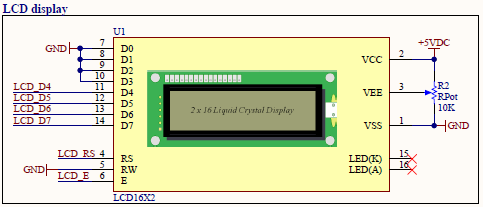
\includegraphics[scale=0.9]{Billeder/LCD.PNG}
			\end{center}
			\label{fig:LCD}
			\caption{LCD pinout}
\end{figure}



\subsubsection{Keypad}

Keypad
I vores Kit er der givet en keypad med 12 knapper fra 0 til 9 og *,\#. Dette keypad virker bare som switches så derfor skal vi selv definere hvad de forskellige knapper skal gøre, for at gøre det simpelt betyder hver knap det som der står på keypaded. Den har to porte til knyttet som er PORT A og PORT E. Det betyder at vi kan læse på PORT E hvis en af GPIO pinden på PORT A er aktiv. [Billede Keypad]
\\
Dette billede kan vi se at vi har givet de forskellige knapper unikke værdier. Dette gøre fordi vi har et array som indeholder alle værdier på keypad’et, som vi så sender kan sende ind i buffer og læse på. For at finde en karakter kigger vi først på alle X værdier (PORT A) igennem og ser om en Y værdi (PORT E) er aktiv og ud fra hvilken X og Y værdi fordi en af tallen på  [Ref billede Keypad].
\\
Dette keypad kan blive brugt til at sende data eller manuelt vil sætte nogle værdier i mens programmet køre.




\subsection{Serial Peripheral Interface}

Microcontrolleren der blev udleveret dette semester (TM4C123GH6PM) indeholder 4 SSI (Synchronous Serial Interface) da disse 4 interfaces alle er ens, på undtagelse deres pins, er SSI0 blevet valgt som interface, dvs. port A pin 2 er til SSI0Clk (modulets clock), pin 3 er SSI0Fss (frame signalet), pin 4 er SSI0Rx (modtagelse), og pin 5 er SSI0Tx (afsendelse)

Til SSI modulet er der 3 forskellige data formater:

\begin{itemize}
	\item Texas Instruments Synchronous Serial
		\begin{figure}[h]
			\begin{center}
			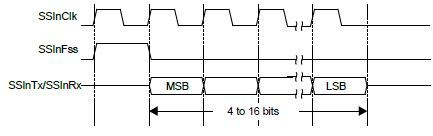
\includegraphics[scale=1]{Billeder/TI_Synchronous_Serial_Frame_Format.jpg}
			\end{center}
			\label{fig:TIFrameFormat}
			\caption{TI Synchronous Serial Frame Format (Single transfer)}
		\end{figure}

	\item Freescale SPI
		\begin{figure}[h]
			\begin{center}
			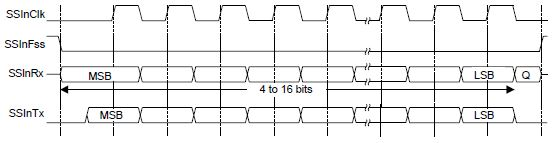
\includegraphics[scale=1]{Billeder/FS_Frame_Format.jpg}
			\end{center}
			\label{fig:FSFrameFormat}
			\caption{FreeScale Frame Format (Single Transfer)}
		\end{figure}
		  
	\item Microwire
		\begin{figure}[h]
			\begin{center}
			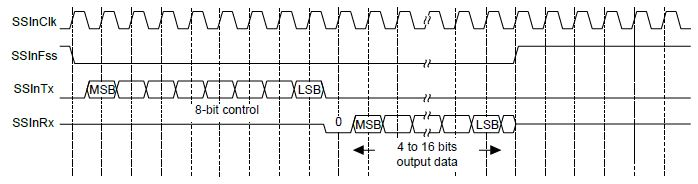
\includegraphics[scale=0.8]{Billeder/MW_Frame_format.jpg}
			\end{center}
			\label{fig:MWFrameFormat}
			\caption{Micro Wire Frame Format (Single Transfer)}
		\end{figure}
\end{itemize}

Da Freescale er den eneste SPI iblandt de tre SSI moduler er det den der blev valgt.

		\begin{figure}[h]
			\begin{center}
			\includegraphics[scale=0.8]{Billeder/Spi_Setup.jpg}
			\end{center}
			\label{fig:SPI_Setup}
			\caption{Setup af Freescale SPI}
		\end{figure}

For at lave et Freescale setup skal der SSI modulet disables, også kan microcontrolleren sættes som master ved at skrive nul til control registret.
derefer skal clock configurations registret sættes til 0 så vi bruger system clocken.
da der ønskes en 2 Mbps clock bruges følgende ligning

\begin{align*}
2*10^6 bps &= \dfrac{16*10^6 Hz}{CPSDVSR * (1 + 0)}\\
CPSDVSR &= \dfrac{16*10^6 Hz}{2*10^6 bps}\\
CPSDVSR &= 8
\end{align*}

Så sættes kontrol registret for SSI0 til 0xF da bit 3:0 angiver data størrelse, 0xF er så 16-bit data. samtidig bliver Freescale SPI sat op da bit 4 og 5 bestemmer frame formatet, og hvis de begge er lave betyder det at Freescale er valgt. 
og igen sættes bit 1 i kontrol registret for SSI1 til høj så SSI'en er enablet
